\section*{Descrizione}

\Par{Verifica e calibrazione del dinamometro}
Poiché non si ha a disposizione un dinamometro calibrato, si è deciso di utilizzare un oggetto elastico.\\
Dunque è necessario avere una molla o un corpo elastico di cui si conosce la costante elastica $k$ così da poter misurare la forza
 che agisce su di esso tramite la misurazione diretta dell'allungamento in accordo con la legge di Hooke.\\ 
 Poiché non tutti gli oggetti elastici seguono la legge di Hooke, è necessario verificare che gli oggetti scelti abbiano un comportamento 
 simile a quello di una molla ideale.\\
Per eseguire questa verifica si misura l'allungamento di un oggetto elastico al variare della massa ad esso applicata.\\ 
Si posiziona quindi l'oggetto elastico, con l'ausilio del filo di nylon, come in figura \ref{fig:figuraVerifica} e si annota la lunghezza 
dell'oggetto in tensione variando la massa applicata, precedentemente misurata con la bilancia digitale.\\
Si misura quindi la lunghezza dell'oggetto elastico a riposo.\\
\begin{figure}[h]
        \centering
        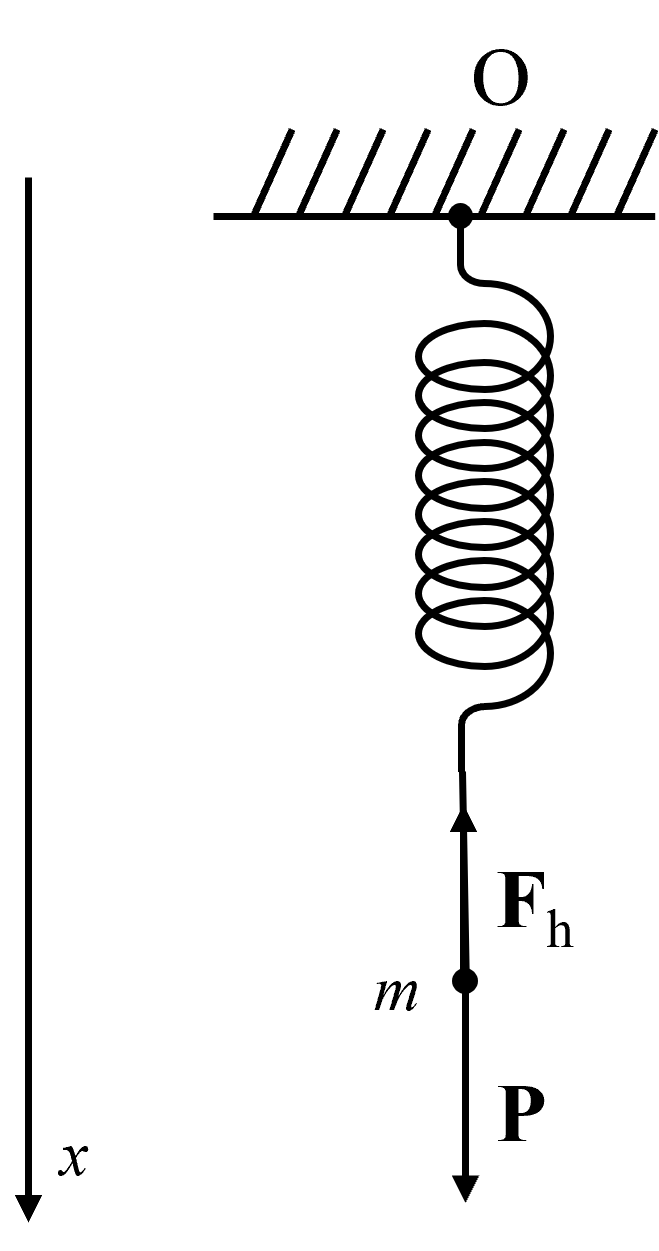
\includegraphics[scale = 0.5]{figures/sch1.png}
        \caption{Configurazione sperimentale per la verifica del comportamento elastico dell'oggetto.}
        \label{fig:figuraVerifica}
\end{figure}
\newpage
\Par{Elaborazione misure per la verifica del dinamometro}
Data la configurazione rappresentata in figura \ref{fig:figuraVerifica}, si osserva che il corpo è in quiete.\\ 
Dunque per i principi della dinamica, la somma delle forze agenti sul corpo è nulla:\\\\
$\vb{P} + \F_h = 0 \qq \rra \qq mg - k(l-l_0) = 0 \qq \rra \qq k = \frac{mg}{l-l_0}$\\ \\
Si riportano le misure effettuate per una elastico di spessore $8\,mm$, una molla di una penna meccanica, e un elastico di spessore $2\,mm$:\\
\begin{table}[h]
    \begin{tabular}{|c|c|c|}
        \hline
        $m$ (massa) & $l$ (lunghezza) & $k$\\
        \hline

        $(117 \pm 1)\; g$  & $(137.0 \pm 0.5) \;mm$ & $(290 \pm 70)\; Nm^{-1}$\\ 
        $(135 \pm 1)\; g$  & $(129.0 \pm 0.5) \;mm$ & $(220 \pm 40)\; Nm^{-1}$\\ 
        $(249 \pm 1)\; g$  & $(148.0 \pm 0.5) \;mm$ & $(163 \pm 11)\; Nm^{-1}$\\ 
        $(387 \pm 1)\; g$  & $(159.0 \pm 0.5) \;mm$ & $(146 \pm 6)\; Nm^{-1}$\\ 
        $(526 \pm 1)\; g$  & $(173.0 \pm 0.5) \;mm$ & $(129 \pm 3)\; Nm^{-1}$\\ 
        $(623 \pm 1)\; g$  & $(183.0 \pm 0.5) \;mm$ & $(122 \pm 2)\; Nm^{-1}$\\ 


        \hline
    \end{tabular}
    \caption{Elastico $8\,mm$ ($l_0 = 133\, mm \pm 0.5\,mm$)}
    \label{tabellaElasitco8}
\end{table}

\begin{table}[h]
    \begin{subtable}[h]{0.45\textwidth}
    \begin{tabular}{|c|c|c|}
        \hline
        $m$ (massa) & $l$ (lunghezza) & $k$\\
        \hline

        $(19 \pm 1)\; g$  & $(25.5 \pm 0.5) \;mm$ & $(400 \pm 500)\; Nm^{-1}$\\ 
        $(64 \pm 1)\; g$  & $(27.5 \pm 0.5) \;mm$ & $(250 \pm 70)\; Nm^{-1}$\\ 
        $(91 \pm 1)\; g$  & $(28.5 \pm 0.5) \;mm$ & $(260 \pm 50)\; Nm^{-1}$\\ 
        $(134 \pm 1)\; g$  & $(29.5 \pm 0.5) \;mm$ & $(290 \pm 50)\; Nm^{-1}$\\ 
        $(181 \pm 1)\; g$  & $(31 \pm 0.5) \;mm$ & $(300 \pm 30)\; Nm^{-1}$\\ 
        $(248 \pm 1)\; g$  & $(33 \pm 0.5) \;mm$ & $(300 \pm 30)\; Nm^{-1}$\\ 
        $(387 \pm 1)\; g$  & $(37 \pm 0.5) \;mm$ & $(316 \pm 18)\; Nm^{-1}$\\ 
        $(526 \pm 1)\; g$  & $(41.5 \pm 0.5) \;mm$ & $(313 \pm 13)\; Nm^{-1}$\\ 


        \hline
        
    \end{tabular}
    \end{subtable}
    \hfill
    \begin{subtable}[h]{0.45\textwidth}
        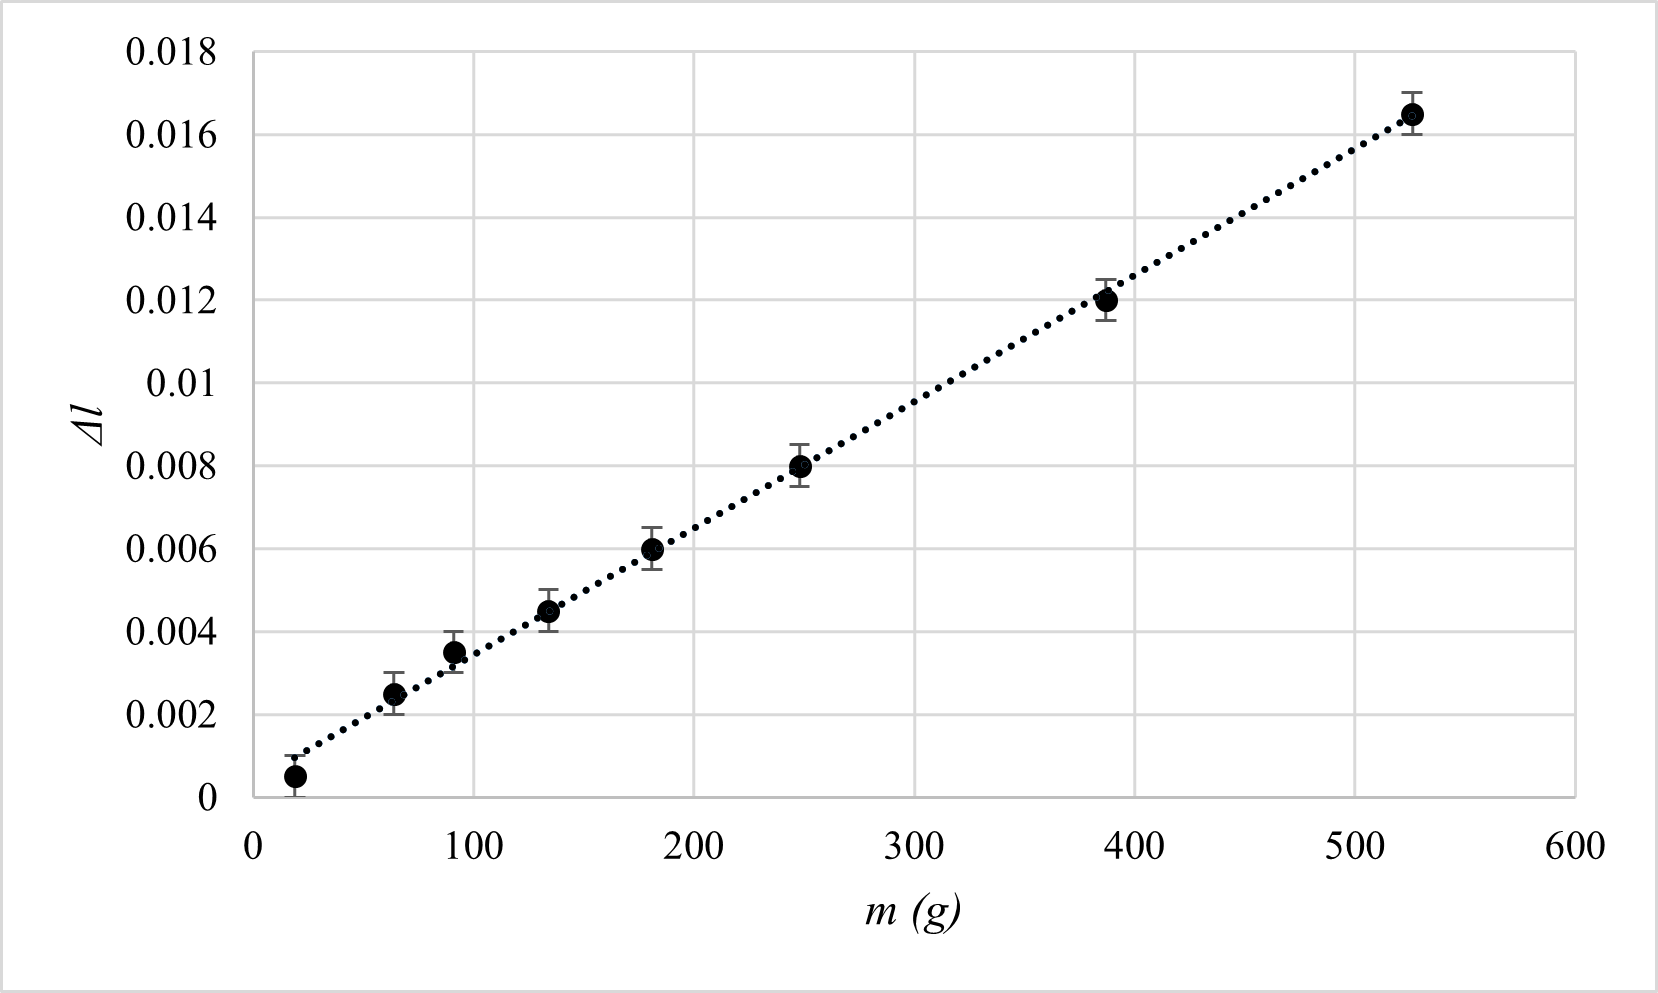
\includegraphics[width = 8cm]{plots/pltMolla.png}
    \end{subtable}
    \caption{Molla ($l_0 = 25.0\, mm \pm 0.5\,mm$) $\qq \sigma_k = 160\; Nm^{-1}$}
    \label{tabellaMolla}
\end{table}


\begin{table}[h]
    \begin{subtable}[h]{0.45\textwidth}
    \begin{tabular}{|c|c|c|}
        \hline
        $m$ (massa) & $l$ (lunghezza) & $k$\\
        \hline

        $(19 \pm 1)\; g$  & $(108.0\pm 0.5) \;mm$ & $(70 \pm 20)\; Nm^{-1}$\\ 
        $(41 \pm 1)\; g$  & $(111.0 \pm 0.5) \;mm$ & $(73 \pm 9)\; Nm^{-1}$\\
        $(64 \pm 1)\; g$  & $(114.0 \pm 0.5) \;mm$ & $(74 \pm 6)\; Nm^{-1}$\\  
        $(74 \pm 1)\; g$  & $(115.5 \pm 0.5) \;mm$ & $(73 \pm 5)\; Nm^{-1}$\\ 
        $(91 \pm 1)\; g$  & $(118.5 \pm 0.5) \;mm$ & $(69 \pm 4)\; Nm^{-1}$\\ 
        $(95 \pm 1)\; g$  & $(119.5 \pm 0.5) \;mm$ & $(67 \pm 3)\; Nm^{-1}$\\ 
        $(134 \pm 1)\; g$  & $(127 \pm 0.5) \;mm$ & $(61 \pm 2)\; Nm^{-1}$\\ 


        \hline
    \end{tabular}
    \end{subtable}
    \hfill
    \begin{subtable}[h]{0.45\textwidth}
        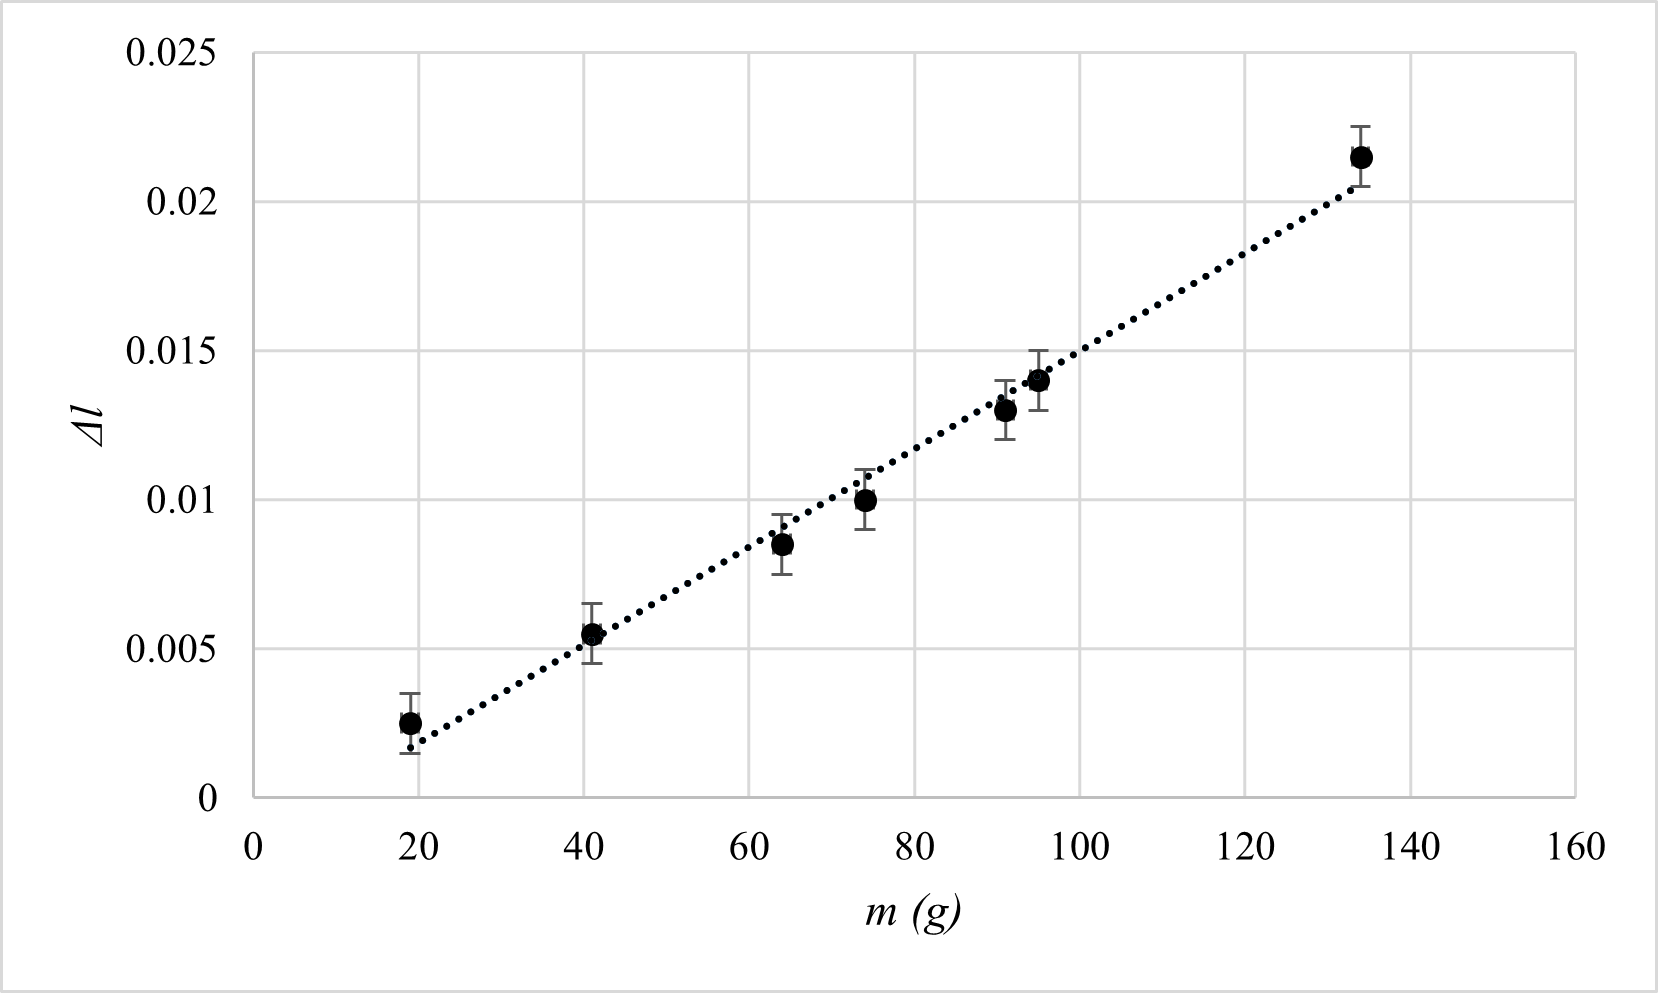
\includegraphics[width = 7cm]{plots/plt2mm.png}
    \end{subtable}
    \caption{Elastico $2\,mm$ ($l_0 = 105.5\, mm \pm 0.5\,mm$)$\qq \sigma_k = 5\; Nm^{-1}$}
    \label{tabellaElasitco2}
\end{table}

Dall'analisi delle costanti elastiche si osserva che l'elastico con spessore di $2\;mm$ è l'oggetto che meglio si comporta come una molla ideale.\\
Per questo motivo si utilizzerà l'elastico di spessore $2\;mm$ come dinamometro per le misure successive
 e si considererà la sua costante elastica paria a $70 Nm^{-1} \pm 5 Nm^{-1}$ .\\
\newpage
\Par{Descrizione esperimento}
Data una superficie fissa, piana e parallela al terreno si posiziono due elastici con lunghezza a riposo e costante elastica note come in figura \ref{fig:figuraEsperimento} 
con l'ausilio di filo di nylon inestensibile\footnote{Il filo si considera inestensibile in quanto, con lo stesso strumento utilizzato durante l'esperimento, non si apprezzano variazioni in lunghezza per tensioni inferiori ai 15 N} e chiodi.\\
Si appende quindi un corpo di massa $m_i$ ai due elastici e si misura la variazione di lunghezza di ciascun elastico.\\
Dopo aver ripetuto le misure variando la massa si misurano gli angoli
$\theta_A$ tra i primo elastico e la superficie piana e $\theta_B$ tra il secondo elastico e la superficie piana.\\
\snls 
\begin{figure}[h!]
        \centering
        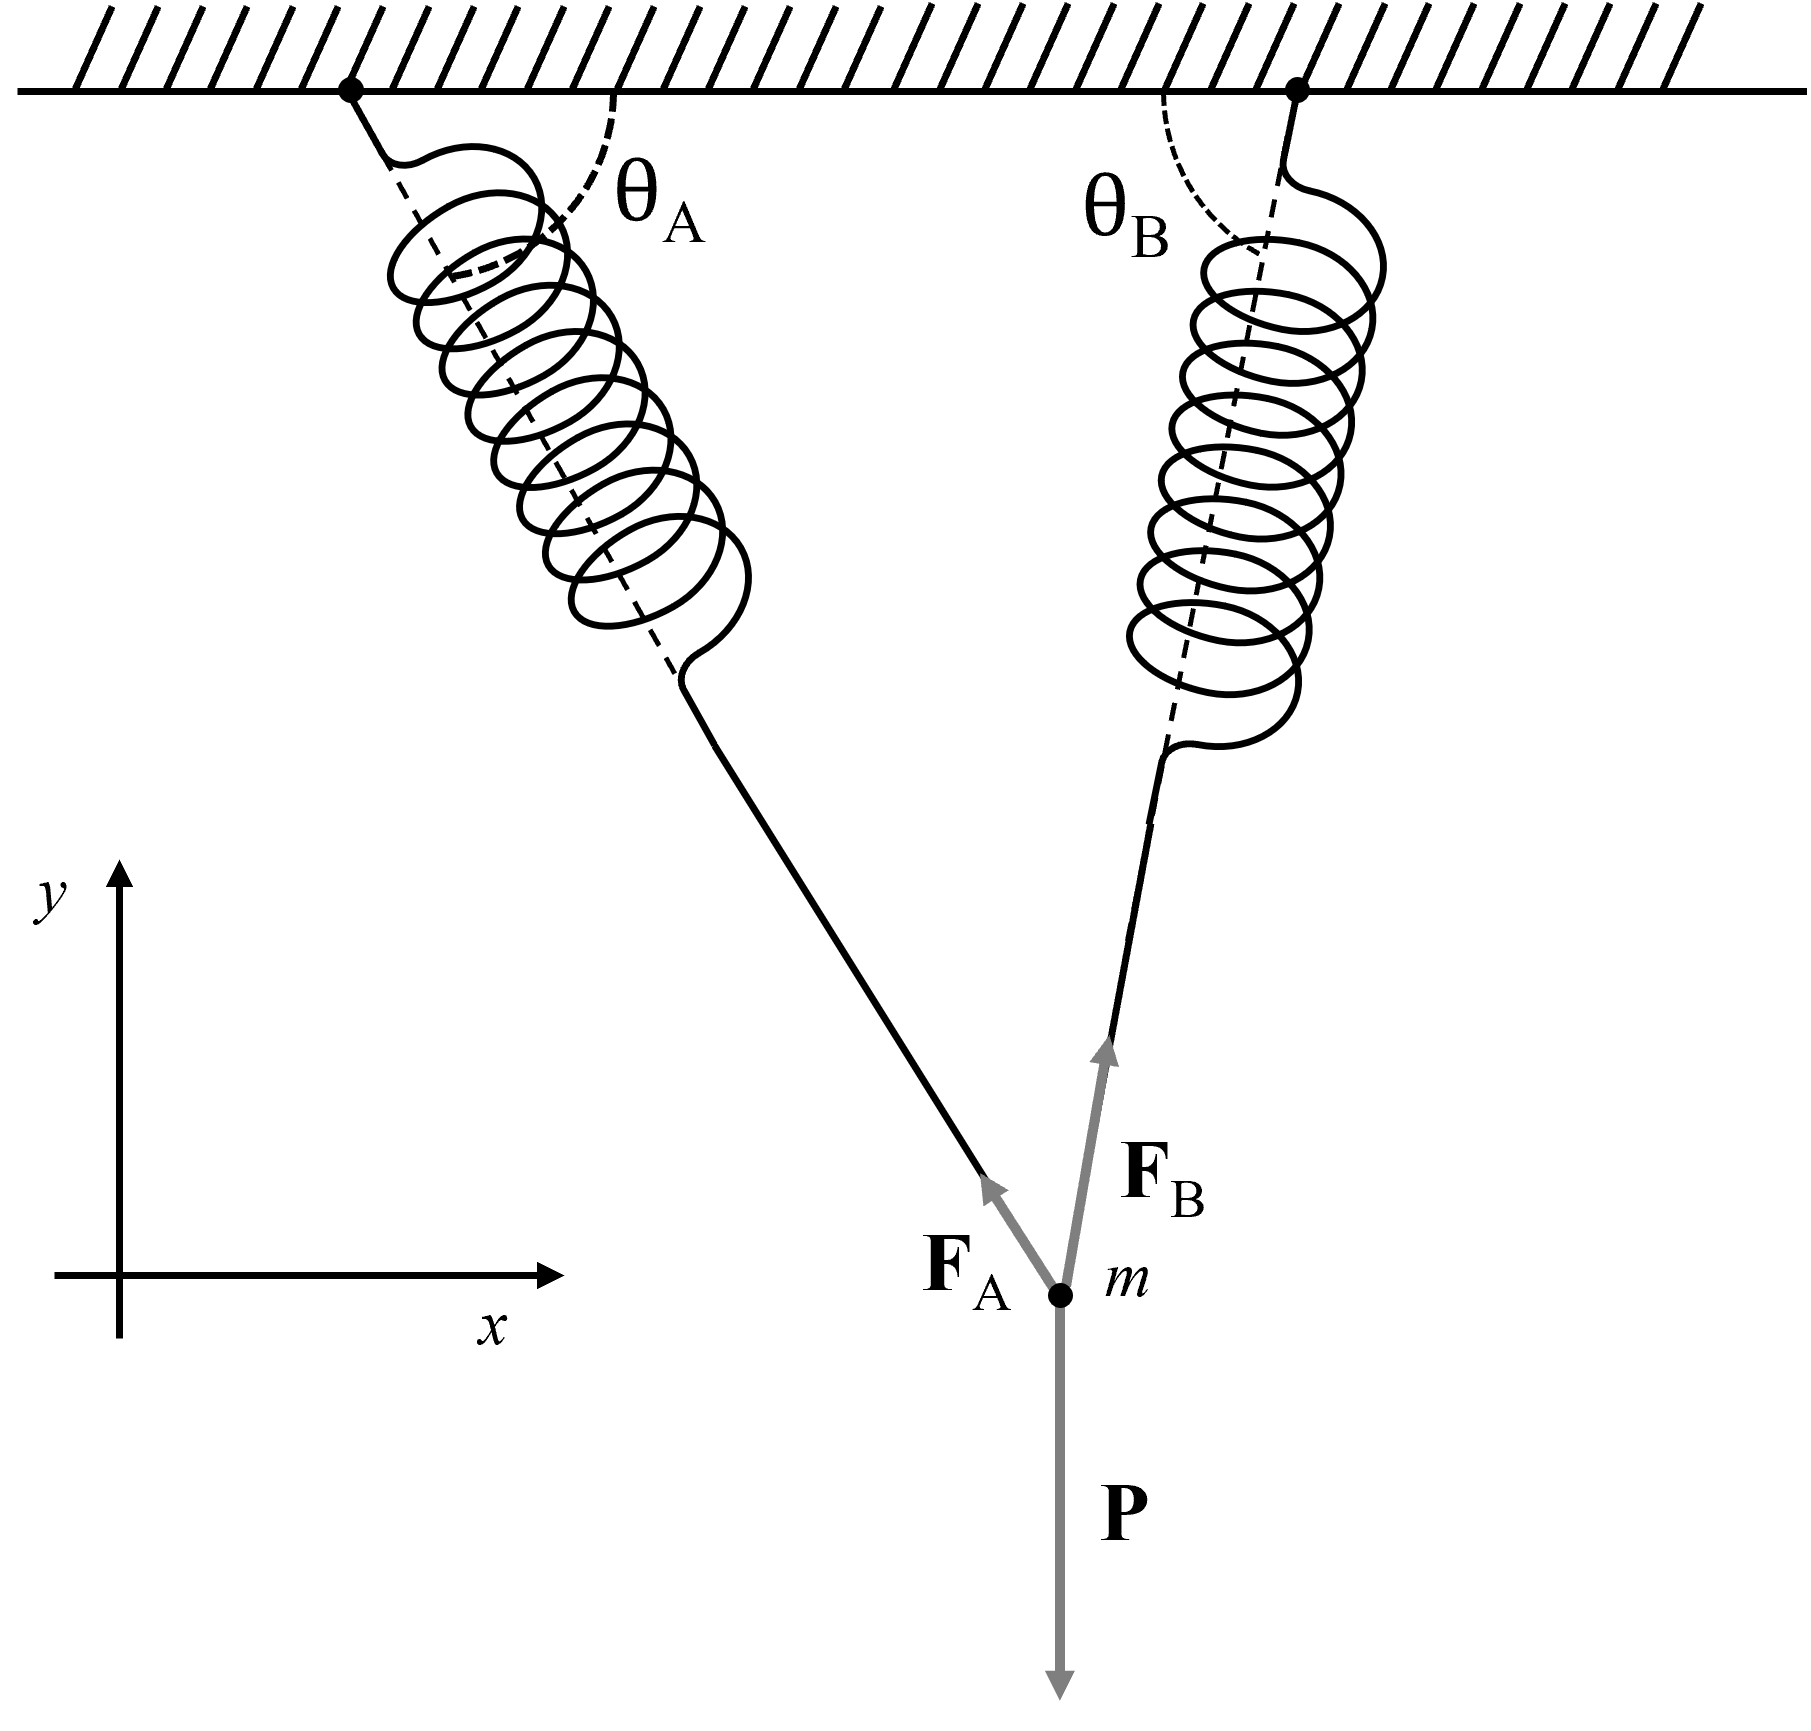
\includegraphics[scale = 0.5]{figures/esperimento.png}
        \caption{Configurazione sperimentale}
        \label{fig:figuraEsperimento}
\end{figure}
